\documentclass[11pt,letterpaper]{article}
\usepackage[margin=0.95in]{geometry}
\usepackage[T1]{fontenc}
\usepackage{amsmath,amssymb,amsthm,booktabs}
\usepackage{tikz,pgfplots}
\usepgfplotslibrary{groupplots}
\pgfplotsset{compat=1.18}
\usepackage[colorlinks=true,linkcolor=blue!45!black,urlcolor=blue!45!black,citecolor=blue!45!black]{hyperref}
\usepackage{microtype}
\newtheorem{proposition}{Proposition}
\newtheorem{corollary}{Corollary}
\newcommand{\E}{\mathbb{E}}
\newcommand{\Prb}{\mathbb{P}}
\newcommand{\ind}{\mathbf{1}}
\setlength{\parindent}{0pt}
\setlength{\parskip}{0.35em}
\setlength{\textfloatsep}{14pt}
\title{Action Efficiency and Initial Moves in Minesweeper}
\author{Minesweeper Exploration\\\small Original analysis and computational checks; not peer reviewed}
\date{October 26, 2026}
\begin{document}
\maketitle
\begin{abstract}
Minesweeper efficiency compares the board's no-flag benchmark, 3BV, with the actions used to solve it. We prove the benchmark formula, derive a local accounting rule for chords, and distinguish a known-board optimum from a policy that must infer hidden mines. A 1,500-board oracle experiment illustrates the savings available from selective chording; exhaustive small-board search demonstrates the limits of greedy choice. A combinatorial corollary establishes that corners maximize the probability of an initial zero under a uniform, first-cell-safe model. This does not establish optimal expected efficiency or even the largest expected first reveal. An independent 90,000-board simulation checks the probability formula and measures revealed area under two protection rules. Guaranteeing a zero removes the corner's zero-probability advantage, and sampled central starts reveal more cells on average. The resulting strategy is objective-dependent: preserve openings, amortize flags across useful chords, and distinguish economy, speed, and survival.
\end{abstract}

\section{The action model and the no-flag benchmark}
Minesweeper Online defines efficiency as 3BV divided by the clicks used to complete a board; flagging and chording can produce values above 100\% \cite{efficiency}. Its gameplay help describes 3BV as the minimum no-flag click count and permits single-click and traditional two-button chords \cite{gameplay}. We use those definitions with explicit discrete accounting: a reveal, flag placement or removal, and chord each cost one action. A two-button chord costs one action. Ineffective actions count; thinking time and cursor travel do not.

Represent the field by an undirected graph $G=(V,E)$, with neighboring cells joined by edges. Classic play uses the eight-neighbor square grid, truncated at the boundary. Fix a mine set $D\subset V$, where $M=|D|<N=|V|$. A safe cell $v$ has clue $n(v)=|N_G(v)\cap D|$. Define
\[
 Z=\{v\notin D:n(v)=0\},\qquad
 I=\{v\notin D:n(v)>0,\ N_G(v)\cap Z=\varnothing\}.
\]
An \emph{opening} is a connected component of $G[Z]$; a zero reveal opens that component and its safe numbered boundary. Let $q$ count openings. The cells in $I$ are isolated from all openings, not necessarily from other numbered cells.

\begin{proposition}[No-flag optimum]\label{prop:nf}
With complete layout knowledge, no flags, and an unrestricted first reveal, the minimum action count is
\begin{equation}\label{eq:bbbv}
 B=q+|I|.
\end{equation}
Every successful no-flag run therefore has $C\geq B$ and efficiency $\eta=100B/C\leq100\%$.
\end{proposition}
\begin{proof}
Each zero component needs a direct reveal within it: it cannot be reached through a different zero component without those components being connected. Each cell in $I$ requires its own reveal because no zero flood reaches it. These are distinct necessities, giving the lower bound. Revealing one zero per component first, then every member of $I$, attains it. Shared numbered boundaries add no unit.
\end{proof}

If a safe first cell $s$ is prescribed, define its numbered opening boundary by
$\partial Z=\{v\notin D:n(v)>0,\ N_G(v)\cap Z\neq\varnothing\}$. Then
\begin{equation}\label{eq:fixednf}
 C^*_{\rm NF}(D;s)=B+\ind\{s\in\partial Z\}.
\end{equation}
A zero or isolated-number start fulfills one necessary action. A boundary-number start fulfills none, leaving all $B$ actions necessary. Thus an initial safe click can still be redundant in the no-flag optimum. Its category, however, is generally hidden from the player.

\section{The marginal value of a chord}
For a fixed board, maximizing $\eta$ is equivalent to minimizing $C$. Write $C^*(D;s)$ for the optimum with flags and chords on a completely known layout and prescribed first reveal. Small instances admit exact unit-cost shortest-path search over revealed-cell and flag states. This is an \emph{oracle} optimization. A real player's choice must depend only on visible observations; different layouts consistent with them can require different best actions.

Suppose an already revealed clue needs $f$ new correct flags to enable a chord. Let $k$ count independent remaining no-flag units completed by that chord: distinct unopened zero components it actually triggers, plus isolated numbers it opens. Several zero neighbors in one component contribute one; a numbered boundary alone contributes zero. Relative to completing those units individually,
\begin{equation}\label{eq:gain}
 \Delta=k-(f+1)
\end{equation}
is the action saving. Thus $\Delta>0$ improves this local comparison, and $\Delta=0$ breaks even. It compares with no-flag completion of those units, not necessarily with another optimal chording plan. Future information, overlapping targets, and flag reuse affect the whole sequence.

\begin{center}\small
\begin{tabular}{p{0.57\linewidth}rrr}
\toprule
Work replaced & $k$ & $f+1$ & $\Delta$\\
\midrule
Three isolated safe numbers; one new flag &3&2&1\\
Two isolated safe numbers; existing flags &2&1&1\\
One whole opening; one new flag &1&2&$-1$\\
Boundary numbers only; one new flag &0&2&$-2$\\
\bottomrule
\end{tabular}
\end{center}

\begin{proposition}[Conservative oracle guarantee]\label{prop:greedy}
Start by revealing a zero. Thereafter either complete one remaining no-flag unit with one reveal, or place $f$ new correct flags and chord only when $k>f+1$. The resulting successful action count satisfies $C\leq B$.
\end{proposition}
\begin{proof}
Let $R$ count unopened zero components plus unrevealed cells in $I$. Initially $R=B$. Each fallback costs one and reduces $R$ by one. Each accepted flag-and-chord block costs $f+1<k$ and reduces $R$ by $k$. Correct flags never obstruct safe floods. Summing costs and reductions until $R=0$ gives $C\leq B$; all safe boundaries have then opened, so the game is complete.
\end{proof}

This guarantee depends on hidden layout knowledge, including which cells belong to openings. Raw revealed area is not $k$. Nor is greedy choice optimal: a shared flag is paid for once across several chords, and a setup reveal with no immediate saving may enable the best later sequence.

\begin{figure}[tb]
\centering
\begin{minipage}[c]{0.43\linewidth}\centering
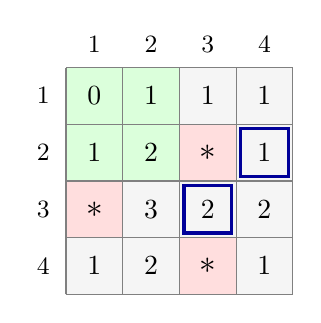
\begin{tikzpicture}[scale=0.72]
\foreach \x in {0,1,2,3} \foreach \y in {0,1,2,3}
 {\fill[gray!8] (\x,-\y) rectangle +(1,-1);}
\fill[green!14] (0,0) rectangle (2,-2);
\foreach \x/\y in {2/1,0/2,2/3}
 {\fill[red!13] (\x,-\y) rectangle +(1,-1);}
\draw[step=1,gray] (0,0) grid (4,-4);
\foreach \x/\y/\v in {0/0/0,1/0/1,2/0/1,3/0/1,0/1/1,1/1/2,3/1/1,1/2/3,2/2/2,3/2/2,0/3/1,1/3/2,3/3/1}
 {\node at (\x+0.5,-\y-0.5) {\v};}
\foreach \x/\y in {2/1,0/2,2/3}{\node[font=\large] at (\x+0.5,-\y-0.5) {$\ast$};}
\foreach \x in {1,2,3,4}{\node[font=\small] at (\x-0.5,0.4) {\x};}
\foreach \y in {1,2,3,4}{\node[font=\small] at (-0.4,-\y+0.5) {\y};}
\draw[very thick,blue!60!black] (3.08,-1.08) rectangle (3.92,-1.92);
\draw[very thick,blue!60!black] (2.08,-2.08) rectangle (2.92,-2.92);
\end{tikzpicture}
\end{minipage}\hfill
\begin{minipage}[c]{0.53\linewidth}\small
\begin{tabular}{rll}
\toprule
Step & Action & (row, column)\\
\midrule
1 & Reveal & (1,1)\\
2 & Reveal & (2,4)\\
3 & Reveal & (4,1)\\
4 & Flag & (2,3)\\
5 & Chord & (2,4)\\
6 & Flag & (4,3)\\
7 & Chord & (3,3)\\
\bottomrule
\end{tabular}
\end{minipage}
\caption{A known-board counterexample to greedy optimality. Green cells open on the first click; stars are mines. One opening and nine isolated numbers give $B=10$. The seven-action sequence scores $142.86\%$ and reuses the flag at $(2,3)$ for the final chord. Blue outlines mark chord centers. The conservative greedy implementation uses ten actions.}
\label{fig:exact}
\end{figure}

Exhaustive breadth-first search on Figure~\ref{fig:exact} finds its first solved state after seven actions, certifying $C^*=7$ for the prescribed start. The search allows every safe reveal, correct flag placement, and productive legal chord. Restricting to correct, persistent flags does not lose a better oracle solution: a safe flag cannot help a successful chord, while removing a correct flag enables neither a safe reveal nor a useful chord. The result is specific to this finite board and action model; it does not make the decisions inferable in blind play.

\section{A paired action-economy experiment}
The companion study evaluates 500 layouts at each standard difficulty with three policies on identical boards. Every policy knows the mines, begins with a guaranteed-zero upper-left reveal, and pays for that reveal. Layouts use a seeded Fisher--Yates shuffle over unprotected cells, with Mulberry32 and finite-resolution scaled integer indices. The comparison isolates action mechanics.

\emph{Random-safe} shuffles safe cells and reveals each still-covered one. \emph{Opening-first} reveals zero components before isolated numbers, attaining $B$. \emph{Selective chords} takes the greatest positive $\Delta$ among revealed clues, with row-major tie-breaking; otherwise it takes the next opening-first move. Previously placed flags are reused without another charge.

\begin{table}[tb]\centering\small
\begin{tabular}{lrrrrr}
\toprule
 & Mean $B$ & Random-safe & No flags & Chords & Actions saved\\
\midrule
Beginner $9\!\times\!9/10$ &15.87&87.44\%&100.00\%&115.04\%&13.93\%\\
Intermediate $16\!\times\!16/40$ &65.37&84.55\%&100.00\%&124.91\%&20.18\%\\
Expert $30\!\times\!16/99$ &174.20&86.09\%&100.00\%&127.79\%&21.79\%\\
\bottomrule
\end{tabular}
\caption{Mean per-board efficiency over 500 paired layouts per row. The last column is the reduction in total actions of selective chords relative to opening-first. An efficiency increase and a percentage of actions saved are different quantities.}
\label{tab:oracle}
\end{table}

All 4,500 policy runs win; every selective-chord run obeys Proposition~\ref{prop:greedy}. Its paired mean improvements are $15.04$, $24.91$, and $27.79$ percentage points. Approximate 95\% intervals, $\bar\delta\pm1.96s_\delta/\sqrt{500}$, are $[13.65,16.42]$, $[23.94,25.88]$, and $[27.07,28.50]$. These measure sampled-layout variation, not uncertainty in human behavior. No losses are discarded.

Mean efficiency is $n^{-1}\sum_i100B_i/C_i$. Pooling gives $100\sum_iB_i/\sum_iC_i$, yielding $116.18\%$, $125.28\%$, and $127.86\%$ for selective chords. Neither is interchangeable with the other. A hidden-information study should also report attempted boards, losses, and failure costs; conditioning only on wins can favor risky policies.

\section{A corollary for the initial click}
The official gameplay help recommends corners for openings \cite{gameplay}. The precise conclusion depends on the generator's protection rule. Moving the first click may change the conditional distribution of complete layouts.

\begin{proposition}[Zero probability under safe-cell conditioning]\label{prop:zero}
Fix a starting cell $s$ of degree $d$. If $M$ mines are uniform among the other $N-1$ cells, then
\begin{equation}\label{eq:pzero}
 p_d=\Prb(n(s)=0\mid s\text{ safe})
 =\frac{\binom{N-1-d}{M}}{\binom{N-1}{M}}
 =\prod_{j=0}^{d-1}\left(1-\frac{M}{N-1-j}\right).
\end{equation}
The binomial ratio is zero when fewer than $M$ eligible cells remain.
\end{proposition}
\begin{proof}
Of the $\binom{N-1}{M}$ equally likely layouts avoiding $s$, exactly $\binom{N-1-d}{M}$ also avoid its neighbors. The product is the equivalent probability that $d$ specified cells are mine-free when sampled without replacement.
\end{proof}

\begin{corollary}[Corner advantage for the event of a zero]\label{cor:corner}
On a classic rectangular field with at least three rows and columns, corners maximize zero probability in the safe-cell model. Their degree is 3, compared with 5 on non-corner edges and 8 in the interior. The ordering is strict when $M>0$ and the compared probabilities are positive.
\end{corollary}
\begin{proof}
In the feasible range,
\[
 \frac{p_{d+1}}{p_d}=\frac{N-1-d-M}{N-1-d}<1\quad(M>0).
\]
Beyond that range additional excluded neighbors keep the probability zero. Hence $p_3\geq p_5\geq p_8$.
\end{proof}

This concerns \emph{getting a zero}, not the expected size of its opening. Fewer neighbors make a corner zero more frequent, while the geometry of a zero's component and boundary can still favor a larger reveal elsewhere.

\textbf{No protection.} Under uniform mines on all $N$ cells, first-click survival is $(N-M)/N$ everywhere. The probability of surviving and being zero is $\binom{N-d-1}{M}/\binom{N}{M}$. The corner improves zero probability, not immediate survival.

\textbf{Zero exclusion.} A generator forbidding mines at $s$ and every neighbor guarantees a zero at every feasible start. There is then no corner advantage in zero probability. Each start excludes a different set of cells and therefore changes the full-layout distribution.

Let $R_s$ count all safe cells opened by the first reveal, including its numbered boundary. An exact decomposition is
\begin{equation}\label{eq:area}
 \E[R_s\mid s\text{ safe}]=1-p_d+p_d\,\E[R_s\mid n(s)=0].
\end{equation}
A positive clue opens exactly one cell. Conditional on zero, uniform safe-cell layouts have precisely the same law as uniform zero-exclusion layouts at that start. Thus a less frequent zero can be offset by a larger conditional opening; maximizing $p_d$ alone does not maximize Equation~\eqref{eq:area}.

Nor does maximizing revealed area establish the best expected efficiency, information gain, survival, or speed. In Equation~\eqref{eq:fixednf}, the extra cost depends on being a \emph{numbered boundary}, not merely on failing to be zero. Moreover $B$ varies by layout, and a large zero opening still counts as one benchmark unit. The corner corollary is not a universal first-move prescription.

\section{Independent simulation checks}
We generated 5,000 layouts for each of three board sizes, three starts, and two protection rules: 90,000 boards. Starts are the top-left corner, top-edge midpoint, and a central cell. In zero-based $(x,y)$ coordinates the latter two are $(\lfloor w/2\rfloor,0)$ and $(\lfloor w/2\rfloor,\lfloor h/2\rfloor)$. Flood counts include revealed boundary numbers, with no flags present.

The implementation is independent of the game and earlier action-policy study. It uses Mulberry32 integer outputs, rejection-sampled bounded integers, and Fisher--Yates sampling. Rejection removes bounded-index bias under ideal uniform 32-bit outputs; finite deterministic PRNG limitations remain. Conditions have disjoint documented seed ranges. Intervals quantify Monte Carlo variation under these assumptions, not uncertainty about an online site's generator.

\begin{table}[tb]\centering\small
\begin{tabular}{llrrr}
\toprule
Board & Start & Exact zero chance & Simulated & 95\% Wilson interval\\
\midrule
Beginner & Corner &66.63\%&67.08\%&65.76--68.37\%\\
 & Edge &50.35\%&50.48\%&49.09--51.86\%\\
 & Center &32.57\%&31.90\%&30.62--33.21\%\\
\addlinespace
Intermediate & Corner &59.80\%&59.34\%&57.97--60.69\%\\
 & Edge &42.29\%&42.90\%&41.53--44.28\%\\
 & Center &25.01\%&24.98\%&23.80--26.20\%\\
\addlinespace
Expert & Corner &49.85\%&49.66\%&48.27--51.05\%\\
 & Edge &31.25\%&31.40\%&30.13--32.70\%\\
 & Center &15.45\%&15.86\%&14.87--16.90\%\\
\bottomrule
\end{tabular}
\caption{Zero probabilities under safe-cell-only protection. All nine exact probabilities lie in the individual 95\% intervals: a consistency check, not simultaneous coverage or proof of generator quality. Under zero exclusion, zero probability is exactly 100\% by construction; all 45,000 such trials satisfy it.}
\label{tab:zero}
\end{table}

\begin{figure}[tb]\centering
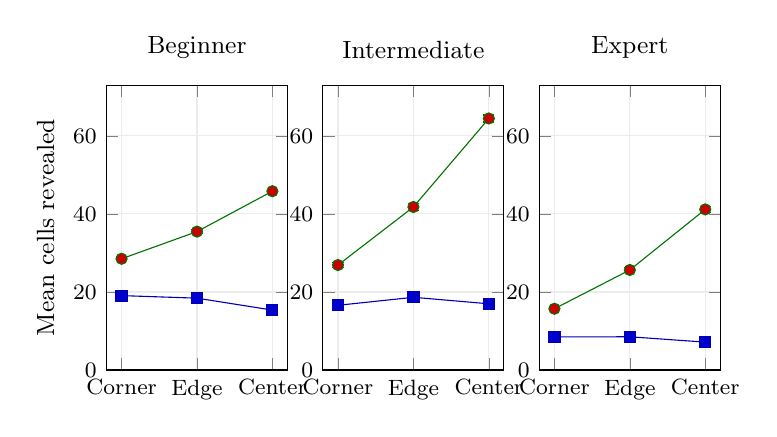
\begin{tikzpicture}
\begin{groupplot}[group style={group size=3 by 1,horizontal sep=0.45cm},width=0.32\textwidth,height=5.2cm,xmin=-0.2,xmax=2.2,ymin=0,ymax=73,xtick={0,1,2},xticklabels={Corner,Edge,Center},tick label style={font=\footnotesize},title style={font=\small},label style={font=\small},grid=major,grid style={gray!15},legend columns=2,legend style={font=\small,draw=none}]
\nextgroupplot[title={Beginner},ylabel={Mean cells revealed},legend to name=openinglegend]
\addplot+[blue!70!black,mark=square*,error bars/.cd,y dir=both,y explicit] coordinates {
(0,19.0698) +- (0,0.5370)
(1,18.4150) +- (0,0.5721)
(2,15.3620) +- (0,0.6101)
};
\addlegendentry{Safe cell only}
\addplot+[green!45!black,mark=*,error bars/.cd,y dir=both,y explicit] coordinates {
(0,28.5088) +- (0,0.5040)
(1,35.4726) +- (0,0.4412)
(2,45.8208) +- (0,0.3212)
};
\addlegendentry{Zero guaranteed}

\nextgroupplot[title={Intermediate}]
\addplot+[blue!70!black,mark=square*,error bars/.cd,y dir=both,y explicit] coordinates {
(0,16.5880) +- (0,0.6590)
(1,18.6364) +- (0,0.7857)
(2,16.9752) +- (0,0.8927)
};
\addplot+[green!45!black,mark=*,error bars/.cd,y dir=both,y explicit] coordinates {
(0,26.9030) +- (0,0.7360)
(1,41.7786) +- (0,0.8456)
(2,64.4530) +- (0,0.9008)
};

\nextgroupplot[title={Expert}]
\addplot+[blue!70!black,mark=square*,error bars/.cd,y dir=both,y explicit] coordinates {
(0,8.4862) +- (0,0.3581)
(1,8.5208) +- (0,0.4199)
(2,7.1482) +- (0,0.4749)
};
\addplot+[green!45!black,mark=*,error bars/.cd,y dir=both,y explicit] coordinates {
(0,15.7024) +- (0,0.3938)
(1,25.6416) +- (0,0.5414)
(2,41.1626) +- (0,0.7092)
};
\end{groupplot}
\end{tikzpicture}
\par\smallskip\ref{openinglegend}

\caption{Mean cells revealed by the first click, with $\bar R\pm1.96s_R/\sqrt{5000}$ intervals. Zero probability and mean revealed area are different objectives. Zero-guaranteed central starts open more cells than corners in all three sampled board classes.}
\label{fig:area}
\end{figure}

For Intermediate safe-only boards, the means are $16.59$ cells at the corner, $18.64$ at the selected edge, and $16.98$ at the center. Thus the most likely position for a zero need not maximize mean revealed area. For Expert, corner and edge means are nearly equal ($8.49$ versus $8.52$); these data do not justify ranking those two area means.

Under zero exclusion, corner/center means are $28.51/45.82$ on Beginner, $26.90/64.45$ on Intermediate, and $15.70/41.16$ on Expert. The Expert corner interval is $[15.31,16.10]$ and center interval $[40.45,41.87]$. These contrasts apply to this model and these cells. We did not optimize over every start, play the resulting games to completion, or measure clue informativeness.

The studies also check Equation~\eqref{eq:area}. The exact Intermediate-center $p_8=0.25010$ and zero-exclusion sample mean $64.453$ imply $16.87$ revealed cells under safe-only protection, close to the independent observed mean $16.98$ (95\% interval $[16.08,17.87]$). This supports the intended relationship between the two sampled conditional distributions.

\section{Efficiency, speed, and practical conclusions}
For a completed board taking time $T$,
\begin{equation}
 \frac{B}{T}=\frac{\eta}{100}\frac{C}{T}.
\end{equation}
This identity relates benchmark units per second, efficiency, and actions per second; it does not imply independent control of them. Fifty units in 40 actions and 30 seconds gives 125\% at 1.67 units/s; 50 actions in 20 seconds gives 100\% at 2.50 units/s. A cheaper action plan can require more thinking or pointer travel.

A hidden-information policy may optimize win probability, expected completion time, or $\E[\eta\mid\mathrm{win}]$. These need not share an optimizer: a higher conditional score may coexist with more failures. State the objective, loss convention, protection rule, and board class before calling a strategy best.

The actionable lesson is to identify safe openings before revealing their borders, place flags when their total future chord savings repay them, and consider setup reveals and flag reuse beyond the immediate chord. The initial-click recommendation is narrower: choose a corner to maximize zero probability under uniform safe-cell-only protection. Under a guaranteed-zero generator, that reason disappears. The best first move for final efficiency requires evaluating the later information-limited policy, not just its initial flood.

\section{Reproducibility and scope}
In the main Minesweeper folder, \texttt{research/experiment.cjs} regenerates the 1,500-board study; \texttt{research/exact-small.cjs} regenerates the finite optimum. Per-board scores and action traces are in \texttt{data/}. In this paper's folder, run
\begin{quote}\small\ttfamily
node initial-position-study.cjs 5000
\end{quote}
to recreate the 90,000-board study, raw CSV, JSON summaries, plotting data, and figure source. Its seed is
\[
\texttt{0x7C190000}+2{,}000{,}000\ell+500{,}000m+100{,}000p+r,
\]
where $\ell,m,p$ index difficulty, protection, and position from zero, and $0\leq r<5000$. Samples are reproducible, not exhaustive. Approximate intervals omit model misspecification and human decision uncertainty. These derivations and computational checks are an original research note, not a reviewed claim of optimal general Minesweeper play.

\begin{thebibliography}{9}
\bibitem{efficiency} Minesweeper Online. \emph{Efficiency}. Official help page. Accessed October 26, 2026. \url{https://minesweeper.online/help/efficiency}.
\bibitem{gameplay} Minesweeper Online. \emph{Gameplay}. Official help page, including chording and 3BV. Accessed October 26, 2026. \url{https://minesweeper.online/help/gameplay}.
\end{thebibliography}
\end{document}
